\documentclass[paper=a4]{article}
\usepackage{ucs}
\usepackage[utf8x]{inputenc}
\usepackage[T1]{fontenc}
\PreloadUnicodePage{0}
\usepackage{xspace}
\usepackage{array}
\usepackage[hmargin=3.5cm,vmargin=2.7cm]{geometry} 
\usepackage{graphicx}


\title{Spillmanual}
\author{Peder Bøen, Kenneth Apeland, Natalie Wannaphong og Joakim Moss Grutle}
\begin{document}
\maketitle

\section{Introduksjon}
Dette er et spill tiltenkt mobiltelefoner der spilleren kjører en bil.
Bilen kjører langs en vei med forskjellige ting i veibanen, som spilleren kan kjøre over eller unngå.
Noen ting vil påvirke spilleren positivt, mens andre kan skade eller ødelegge bilen og avslutte runden.
Spilleren får en score for hver spillrunde, i tillegg til at spilleren samler opp virtuelle penger som kan brukes til å oppgradere bilen.
\begin{center}
\begin{tabular}{ | m{5cm} | m{8cm} | }
\hline
Målgruppe. & Ungdom 15-25 år. \\ \hline
Spillvarighet. & Spillet varer helt til bilen går tom for bensin eller til spilleren kræsjer.\\&
Dette kan ta alt fra få sekunder til mange minutter, da spiller kan plukke opp mer bensin på veien,
oppgradere bensintanken eller kræsje med en gang.\\ \hline
Spillere. & En-spiller spill. \\ \hline
Åpne data. & Bruke åpne data fra yr.no om været og natt/dag. Om det er kaldt kan det være is på veiene\\&
eller om det regner kan dette påvirke kjøreegenskapene. Når det er natt vil det være zombier istedenfor businessmenn\\ \hline
\end{tabular}
\end{center}

\section{Brukermønster}
\begin{figure}\begin{center}
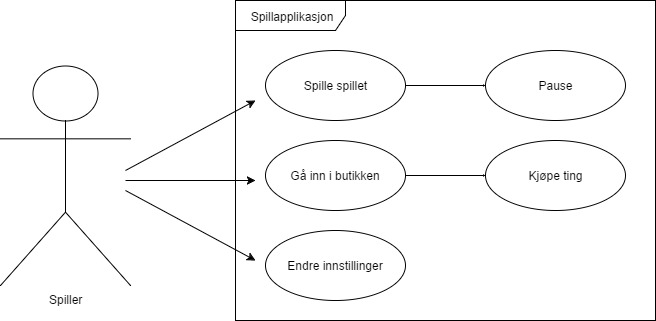
\includegraphics[width=0.75\textwidth]{Use-case.jpg}
\caption{Use-case diagram av spillet}
\end{center}\end{figure}

\begin{center}
\begin{tabular}{ | m{4cm} | m{10cm}|} 
\hline
Pre-condition & 
Spillet er startet \\&
\\ \hline

Standard path & 
S01 Bruker står i starmenyen \\&
S02 Trykker `play` \\&
S03 Spillet starter \\&
S04 Bruker holder inne til høyre eller venstre for å styre \\&
S05 Bruker unngår hindringene \\&
S06 Bruker plukker opp myntene\\&
S07 Bruker plukker opp bensintankene dersom det kommer\\&
S08 Bruker spiller til tom for bensin \\&
S09 Spillet stopper \\&
S10 Spillet viser high-score og ekstra penger \\&
S11 Spillet lagrer \\&
S12 Spillet går tilbake til startskjermen \\&
\\ \hline

Post-condition & 
Spillet er klar til å avsluttes eller starte på nytt \\&
\\ \hline

Alternative Path & 
A01: @S01, Bruker kan trykke på oppgrader knappen\\& 
		A01.01 Bruker kjøper oppgraderinger dersom han vil\\&
		A01.02 Bilen i spillet blir bedre \\&
		A01.03 Bruker trykker på tilbake-knappen \\&
		A01.04 RESUME @S01 \\&
		\\&
A02: @S01, Bruker kan trykke på tannhjul knappen\\& 
		A02.01 Bruker endrer på instillingene han vil\\&
		A02.02 Spillet godtar instillingene \\&
		A01.03 Bruker trykker på tilbake-knappen \\&
		A02.04 RESUME @S01 \\&
		\\&
A03: @S04-07, Bruker kan når som helst trykke på pause mens han spiller spillet\\&
		A03.01 Spillet settes på pause \\& 
		A03.02 Bruker kan trykke `Avslutt` eller `Fortsett`\\& 
		A03.03 Dersom bruker trykker på `Avslutt`\\& 
		A03.04 RESUME @S09 \\&
		
\\ \hline
\end{tabular}
Use-case: Spille spillet
\end{center}

	\section{Spillregler}
		\subsection{Kontroll}
		\begin{itemize}
			\item{Spilleren kan styre bilen til høyre og venstre.}
			\item{Spilleren kan ikke styre bilens hastighet direkte.}
			\item{Bilen kan ikke styres av veien.}
		\end{itemize}

		\subsection{Objektinteraksjon}
		\begin{itemize}
			\item{Bilen kan treffe objekter i veien.}
			\item{Objekter kan påføre bilen en positiv, eller negativ effekt.}
			\item{Noen objekter kan ødelegge bilen og avslutte runden.}
		\end{itemize}

		\subsection{Poeng}
		\begin{itemize}
			\item{Spilleren tjener poeng hver runde.}
			\item{Poeng blir opptjent avhengig av hvor langt spilleren kjører og hvilke objekter spilleren kjører over.}
			\item{Spilleren starter alltid med 0 poeng i starten av en runde.}
		\end{itemize}

		\subsection{Penger}
		\begin{itemize}
			\item{I slutten av hver runde får spilleren penger i form av spillets egen valuta.}
			\item{Hvor mye penger spilleren får er avhengig av poengscore og objektene spilleren har plukket opp.}
			\item{Pengene kan brukes i spillets butikk fra hovedmenyen for å oppgradere bilen.}
		\end{itemize}

	\section{Brukerhistorier}
		\begin{itemize}
			\item{Som spiller vil jeg ha mulighet til å styre bilen for å kunne velge hva jeg vil kjøre over.}
			\item{Som spiller vil jeg ha mulighet til å sette spillet på pause når jeg vil for å kunne gjøre andre ting.}
			\item{Som spiller vil jeg ha mulighet til å avslutte spiller når jeg vil i tilfelle jeg ikke har tid til å spille mer.}
			\item{Som spiller vil jeg ha mulighet til å oppgradere bilen min for å få en følelse av progressjon.}
			\item{Som spiller vil jeg ha mulighet til å se mine høyeste poengscore for å kunne måle min egen progressjon i spillet.}
			\item{Som spiller vil jeg ha mulighet til å justere lydvolumet på spillet for å ikke vere forstyrrende på bussen.}
		\end{itemize}

	\newpage
	\begin{figure}\begin{center}
		\includegraphics[width=1.00\textwidth]{Spillrunde.png}
		\caption{Skisse av en spillrunde.}
	\end{center}\end{figure}

\begin{figure}
\section{Spillillustrasjon}
\begin{center}
\includegraphics[width=1.2\textwidth]{storylineoblig112.png}
\caption{Illustrasjon av fremgangen i spillet}
\end{center}\end{figure}

\begin{figure}
\begin{center}
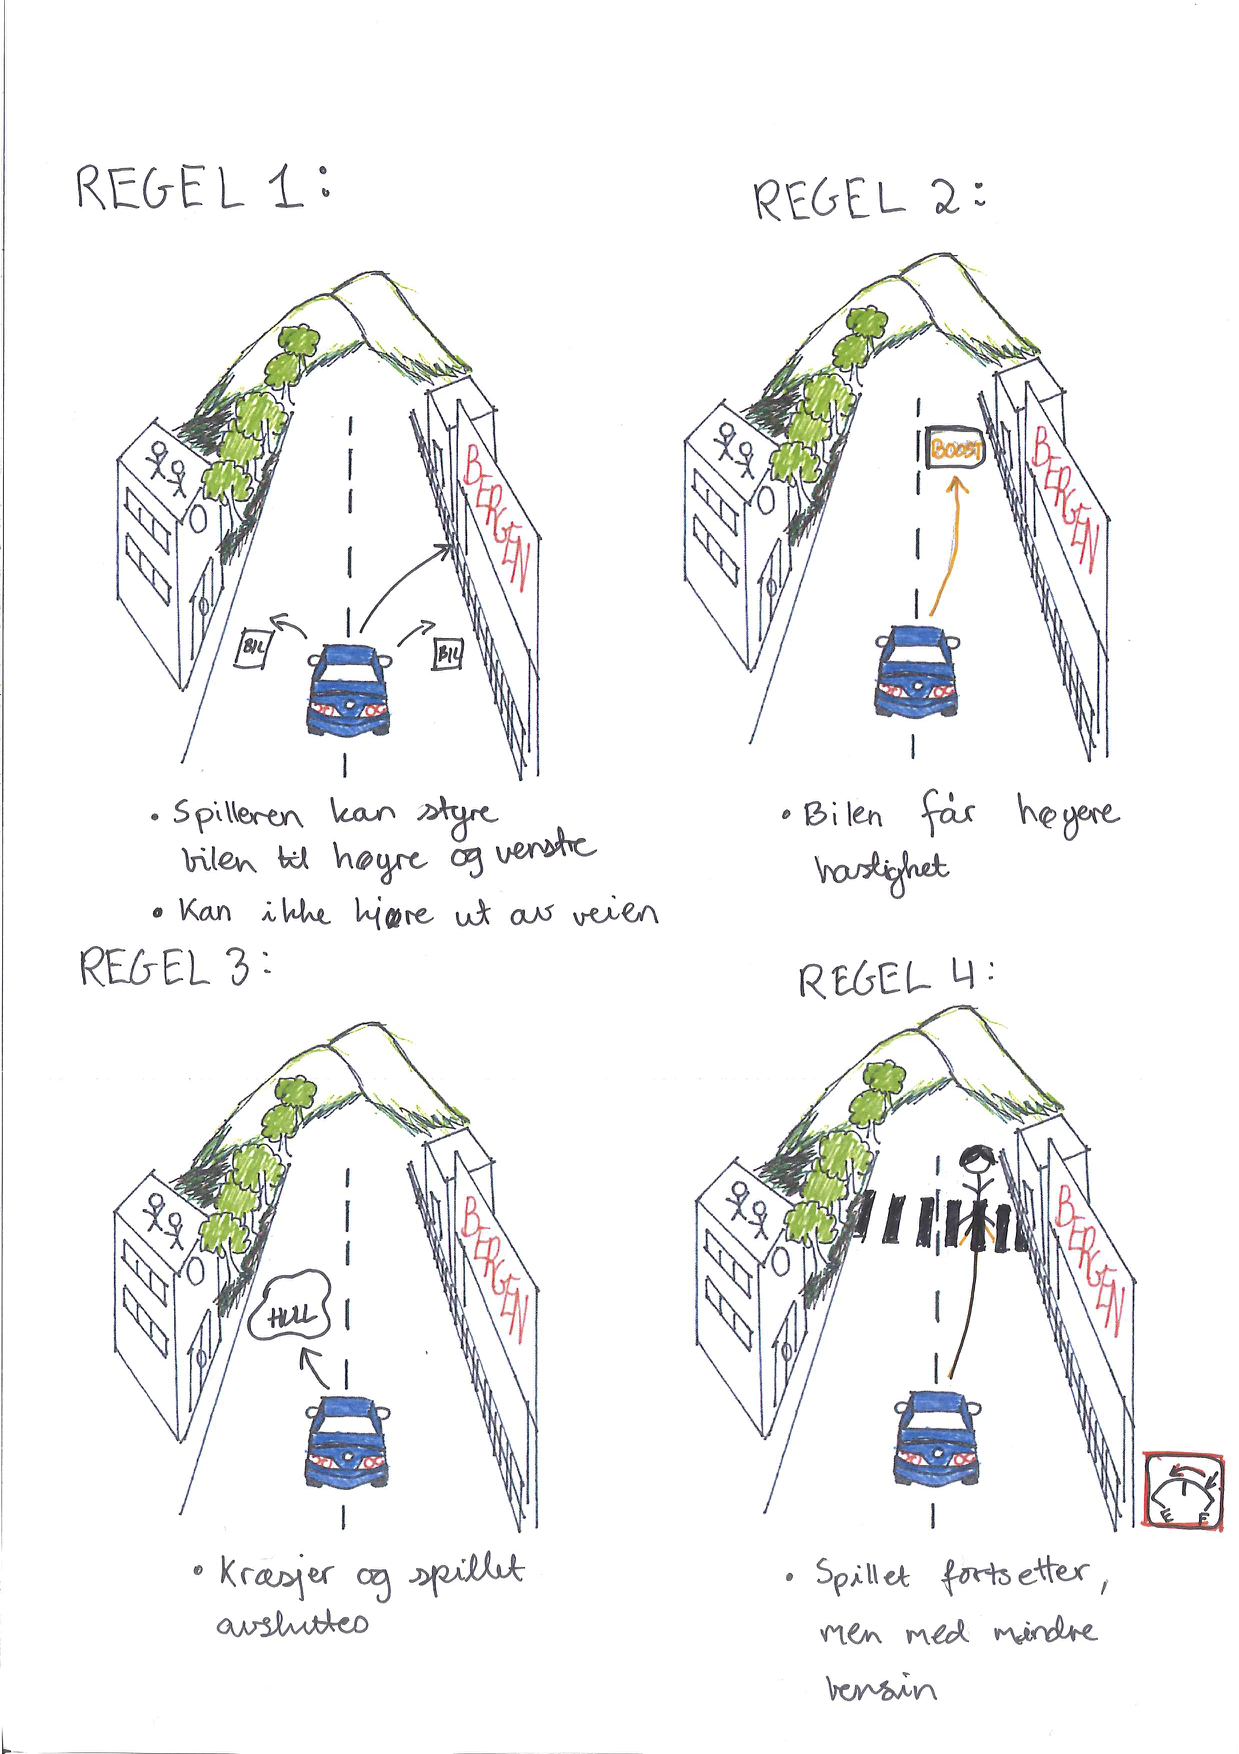
\includegraphics[width=0.50\textwidth]{skisseRegelFixed.png}
\caption{Illustrasjon av fremgangen i spillet}
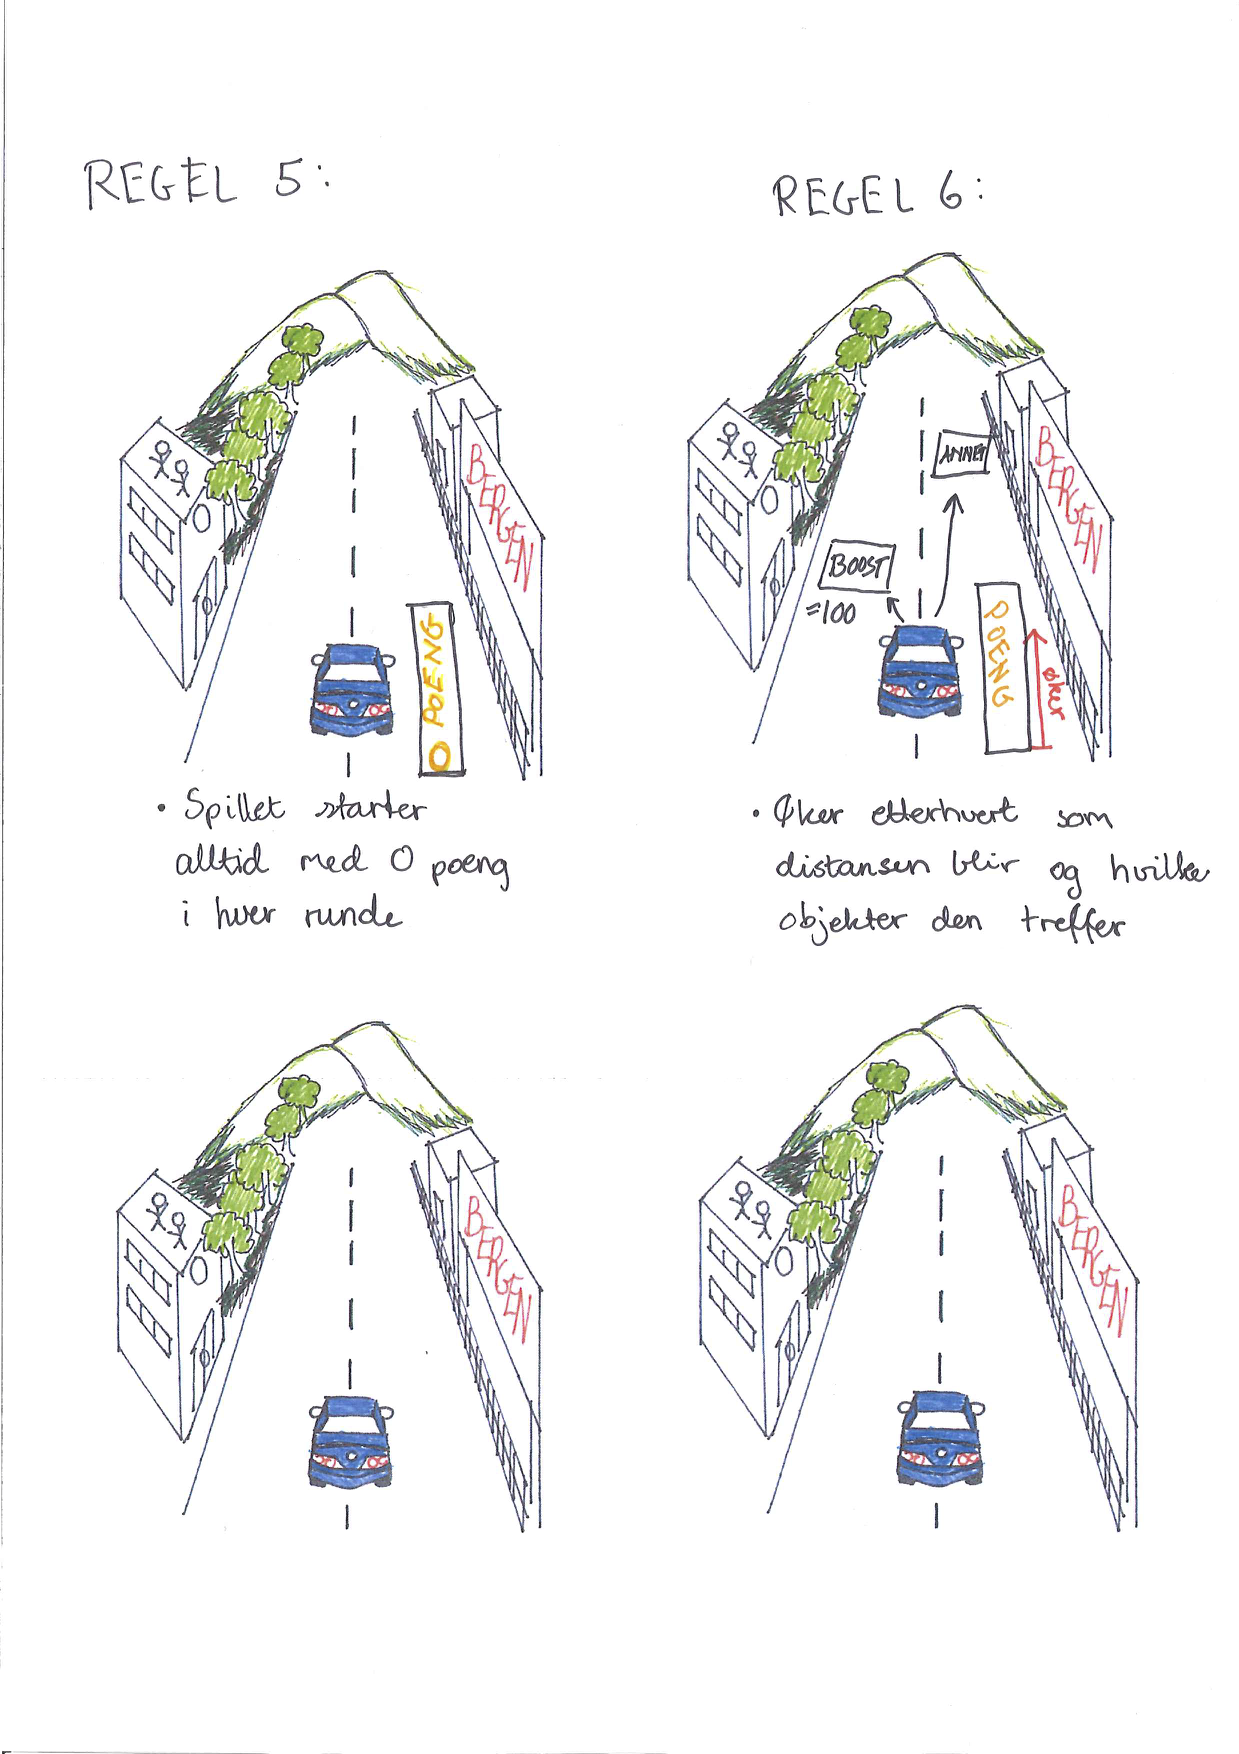
\includegraphics[width=0.50\textwidth]{skisseRegelFixed2.png}
\caption{Illustrasjon av fremgangen i spillet}
\end{center}
\end{figure}


\end{document}